  
\chapter{MARCO CONCEPTUAL}

%=====================================
\section{REDES DE \'AREA LOCAL (LAN)}
En el libro de Tanenbaum hace referencia a una clasificaci\'on basada en la distancia y con un ejemplo mas del mundo real.
\begin{caja}[]{
 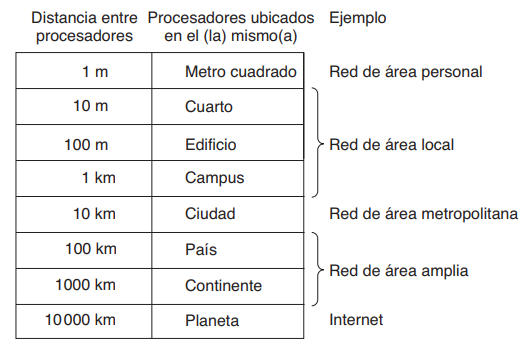
\includegraphics[scale=0.70]{clasifred}
 }\end{caja}
 Seg\'un el gr\'afico una red lan comprender\'ia un cuarto, edificio o campus. Adem\'as Tanenbaum nos menciona que estas redes son de propiedad privada y son utilizadas ampliamente para compartir recursos e intercambiar informaci\'on.\\
 Cuando las empresas usan las redes lan se les conoce como REDES EMPRESARIALES.

Mayormente en los hogares se opta por las conexi\'ones inalambricas

\begin{caja}[]{
 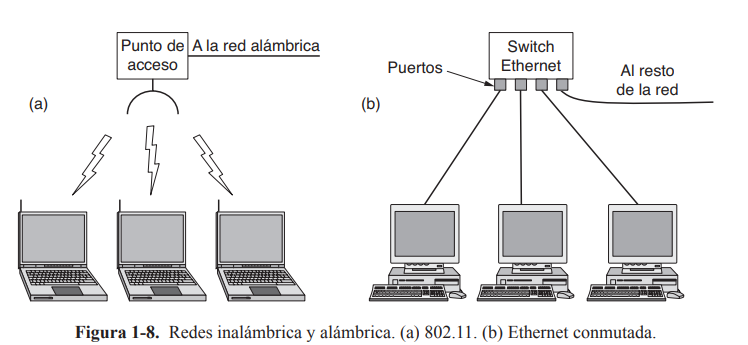
\includegraphics[scale=0.50]{CONEC}
 }\end{caja}
 
Existe un est\'andar para las redes LAN inal\'ambricas llamado IEEE 802.11, mejor conocido como WiFi que opera a velocidades desde 11 hasta cientos de Mbps.
\\
Mientras que para las redes al\'ambrica existe el est\'andar IEEE 802.3, com\'unmente conocido como Ethernet

\\

\begin{definicion}[]
{
Para crear redes LAN m\'as grandes se pueden conectar switches entre s\'i mediante sus puertos.
}
\end{definicion}}
%=====================================0

%========================================
\section{SWICH O CONNMUTADOR}
El trabajo del switch es transmitir paquetes entre las computadoras conectadas a \'el, y utiliza la direcci\'on en cada paquete para determinar a qu\'e computadora se lo
debe enviar. 

%==============================================0

%==============================================
\section{DIRECCI\'ON F\'ISICA MAC (Media Access Control)}
Es un identificador \'unico, son llamadas tambi\'en \textbf{burned-in addresses} ya que son escritas directamente y en forma binaria al momento de la fabricaci\'on del dispositivo.

\begin{definicion}[]
{
Es un identificador de 48 bits donde los primeros  24 bits corresponden al fabricante y los \'ultimos 24 bits es regulada por la IEEE.
\\
la IEEE maneja 3 identificadores globales \'unicos \textbf{MAC-48, EUI-48, y EUI-64}

\end{definicion}}

\begin{caja}[]{
 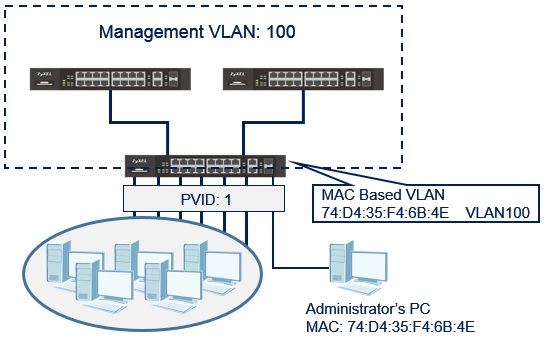
\includegraphics[scale=0.68]{mac}
 }\end{caja}

%==============================================0



\section{HUB O CONCENTRADOR}

\parbox{4cm}{
\begin{caja}[]{
 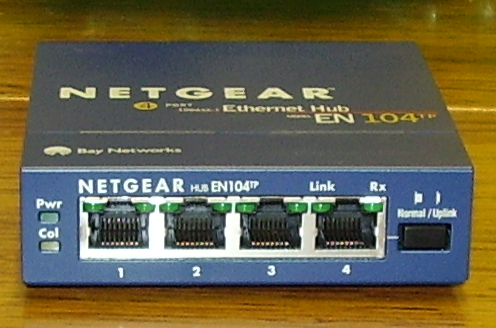
\includegraphics[scale=0.80]{hub}
 }\end{caja}
 } \parbox{10.8cm}{ 
\begin{definicion}[]
{
Trabaja en la capa f\'isica (capa 1) del modelo OSI o la capa de acceso al medio en el modelo TCP/IP. 
\\
Recibe una se\~nal y la repite por sus diferentes puertos.
\\
Actualmente la tarea de los concentradores lo realizan los conmutadores y son m\'as baratos; por ello, los hubs son dificiles de encontrar.
}
\end{definicion}}
\\
